% ===========================================================================
\section{Validation against CLASS}\label{sec:validation}
% ===========================================================================

As an end-to-end test, we ran CLASS~\cite{Lesgourgues2011,Blas2011} (through its Python wrapper) with the same
parameters and physics: massless neutrinos and the same tanh reionization, unlensed unless stated otherwise. This
section uses the Peebles recombination model of Sec.~\ref{sec:m2}; with RECFAST (Sec.~\ref{sec:recfast}), the
code's default, the recombination-driven differences below drop by an order of magnitude in TT and by a factor of four in EE. The comparison
(Fig.~\ref{fig:class}) is:
\begin{itemize}
\item \textbf{Background.} $H$, $t$ and $\eta$ agree to $\sim10^{-7}$. The age (13.8483\,Gyr) and $\eta_0$
      ($14\,191.6\Mpc$) agree in all printed digits.
\item \textbf{Recombination.} CLASS uses HyRec, which includes the multi-level atom and non-equilibrium helium
      recombination. Our $X_e$ agrees to $\sim0.1\%$ during hydrogen recombination. It differs by 3--4\% during
      He$^+$ recombination at $z\approx2000$--$2500$, where our Saha helium recombines too fast, and by $+15\%$ in the
      freeze-out tail. These differences have little effect on the observables:
      \begin{itemize}
      \item $z_*=1084.32$ versus $1084.70$, and $r_s(z_*)=144.90$ versus $144.87\Mpc$;
      \item $z_d=1059.83$ versus $1060.03$, and $r_s(z_d)=147.08$ versus $147.06\Mpc$;
      \item $\tau_{\rm reion}=0.0580$ versus $0.0578$.
      \end{itemize}
\item \textbf{Angular spectra.}
      \begin{itemize}
      \item TT agrees to $1.1\%$ for $2\le\ell\le2000$, and to $0.97\%$ for $\ell\le1200$.
      \item EE agrees to $1\%$ at $\ell=2$--8 and to $3.4\%$ for $\ell\ge100$. The largest difference, up to $+6\%$, is
            in the EE trough at $\ell\approx15$--20, where the spectrum is tiny.
      \item TE differs by at most $1.5\%$ of its peak amplitude.
      \end{itemize}
      When we remove helium from both codes, TT agrees to 0.3--0.9\%. The remaining differences are therefore mostly
      due to the recombination model, which changes the damping tail and the polarization amplitude.
\item \textbf{Matter power spectrum.} $P(k)$ agrees to $0.11\%$ for all $k$.
\item \textbf{Lensing.} To separate the lensing from the unlensed spectra we compare the ratio of lensed to unlensed
      spectra from each code, with CLASS run with lensing on and $\Delta\ell=500$ extra multipoles. The TT ratios
      agree to $1.2\times10^{-4}$ for $\ell\le1000$, $5.8\times10^{-4}$ for $\ell\le2000$ and $1.1\times10^{-3}$ for
      $\ell\le2500$. $C_\ell^{\phi\phi}$ agrees to $0.11\%$ for $\ell\le1000$ and $1.1\%$ up to $\ell=2500$, where our
      extrapolation of the Weyl potential beyond $k_{\max}$ takes over. The lensing B modes agree to $1.5\%$ for
      $\ell\le2000$ and $1.2\%$ up to $\ell=2500$. Fed with identical input spectra, our lensing module reproduces CLASS's lensed TT to $1.4\times10^{-4}$.
\end{itemize}

\begin{figure*}
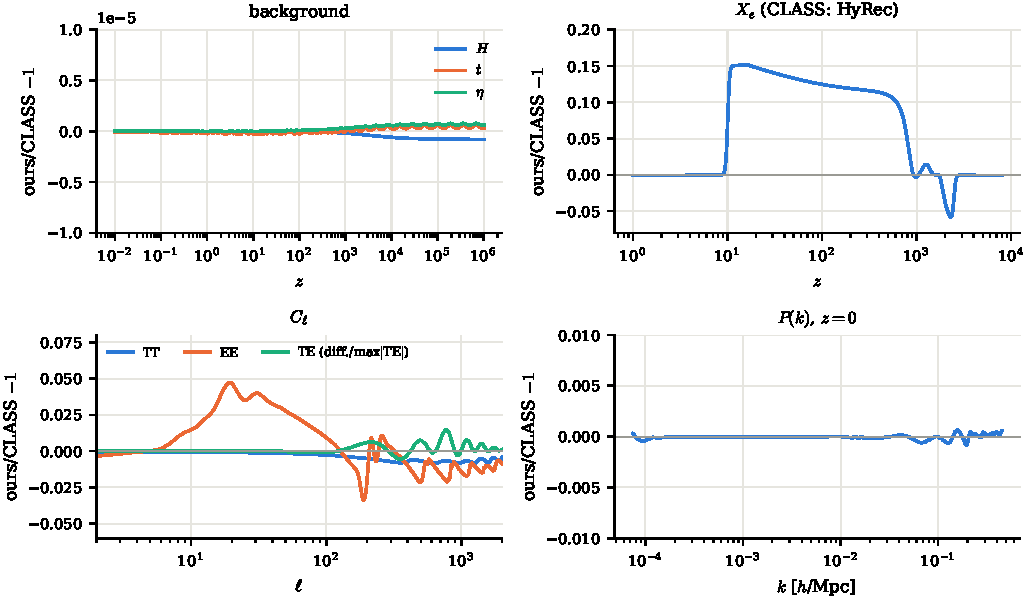
\includegraphics[width=0.9\textwidth]{validation_class}
\caption{Relative differences between our code and CLASS run with the same physics. \emph{Top left:} background
$H$, $t$ and $\eta$. \emph{Top right:} free electron fraction (CLASS uses HyRec). \emph{Bottom left:} unlensed TT
and EE spectra, and the TE difference relative to the maximum of $|C_\ell^{TE}|$. \emph{Bottom right:} matter power
spectrum today.}
\label{fig:class}
\end{figure*}
